\chapter{Testing and evaluation}

This chapter presents details of the implementations, experiments and evaluations for the Delta robot and testing system in previous chapter. Section 1 describes the experimental environment, which include hardware and supporting hardware. Subsequently, section 2 presents all the experiments along with evaluation and assessment. In the final section, conclusions are presented to the end of this chapter.

\section{Experimental environment}
\subsection{Hardware configurations}
In accuracy and stability test, only Delta robot is enough for the test. The tests for the automated mobile app testing system are conducted with the hardware configurations as shown in table \ref{tab:hw}. We use 2 phones running 2 different \acrshort{os} versions with different screen size and resolution for testing the portability of the system.

\begin{table}[H]
	\centering
	\caption{Hardware configuration for testing process}	
	\label{tab:hw}
	\begin{tabularx}{0.65\textwidth}{ll}
		\toprule
		Phone 1 & ASUS Zenfone 5 \\
			  & Resolution 720 x 1280 pixels \\
			  & Screen 5'' 6.22 cm x 11.06 cm \\
			  & Android 5.0.1\\
		\midrule 
		Phone 2 & Sony XPeria L \\
			  & Resolution 480 x 850 pixels \\
			  & Screen 4.3'' 5.40 cm x 9.60 cm \\
			  & Android 4.2.2\\
		\midrule 
		Robot & Self-construct Delta Robot \\
			  & \begin{minipage}{0.5\linewidth}
				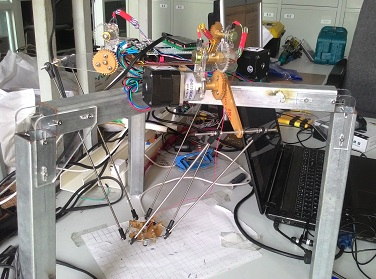
\includegraphics[width=0.8\linewidth]{Chapters/Fig/real_delta_robot.jpg}
				\end{minipage} \\
		\midrule 
		Computer & Windows PC \\
		\bottomrule
	\end{tabularx}
\end{table}

\subsection{Software}

In the test for automated mobile app testing system, beside running testing application, we are required to have the following software installed on the computer.

	\begin{itemize}
		\item[--] \textbf{Android platform tool}: command line tools for communicate with Android device.
		\item[--] \textbf{Droid@Screen}: application letting us capture Android screen to PC.
		\item[--] \textbf{Simple Click Test}: self-created tested application for Experiment 1.
		\item[--] \textbf{Clock ICS}: tested application for Experiment 2. This application can be downloaded on Google Play Store \footnote{Available at: \url{https://play.google.com/store/apps/details?id=com.moblynx.clockics}}
	\end{itemize}

\section{Testing and evaluation}

This section gives the details of all experiments that I have conducted to explore and evaluate accurate and stability of Delta robot, as well as it's feasibility in the real environment.

\subsection{Experiment 1: Test robot accuracy}
\subsubsection{Experiment's purpose}
Check the accuracy of the Delta Robot when moving to some points in workspace.
\subsubsection{Experimental setup}
Open test application, use control API to move end effector to a point.
\subsubsection{Experimental result and evaluations}
\begin{table}[H]
	\centering
	\caption{Experimental 1 result}	
	\label{tab:experiment_1}
	\begin{tabularx}{0.4\textwidth}{l|l}
		\toprule
		\textbf{Destination}	& \textbf{Real Coordinate} \\
		\midrule 
		$(0,0,-270)$			& $(0,0,-270)$ \\
		\midrule 
		$(10,0,-270)$			& $(10,0,-270)$ \\
		\midrule
		$(20,0,-270)$			& $(20,0,-270)$ \\ 
		\midrule
		$(40,0,-270)$			& $(39,0,-270)$ \\ 
		\midrule
		$(80,0,-270)$			& $(79,0,-272)$ \\ 
		\midrule
		$(0,10,-270)$			& $(0,10,-270)$ \\ 
		\midrule
		$(0,20,-270)$			& $(0,19,-270)$ \\ 
		\midrule
		$(0,40,-270)$			& $(0,39,-270)$ \\ 
		\midrule
		$(0,80,-270)$			& $(0,78,-271)$ \\ 
		\bottomrule
	\end{tabularx}
\end{table}

%Robot hoạt động chính xác ở phần gần với trục Z, càng xa trục Z(x, y càng lớn) thì robot hoạt động càng kém chính xác hơn.
The accurate of robot depend on the z-axis. The closer end-effector is to the z-axis the more accurate it operates.

\subsection{Experiment 2: Test robot repeatability}
\subsubsection{Experiment's purpose}
Check the stability of the Delta Robot when running the test script repeatedly.
\subsubsection{Experimental setup}
Open test application, use control API to move end effector to a point and back repeatedly. Specifically, I move the end efector of Delta Robot from point $(-8, 0, -270)$ to $(-8, 0, -270)$ and back 10 times.

\subsubsection{Experimental result and evaluations}
% \begin{table}[H]
% \centering
% \caption{Experimental 2 result}
% \label{tab:experiment_2}
% \begin{tabular}{|l|l|l|}
% \hline
% \multirow{2}{*}{Times} & \multicolumn{2}{l|}{Value of potentiometer} \\ \cline{2-3} 
%                        & (-80, 0, -270)        & (80, 0, -270)       \\ \hline
% 1                      & 526:288:490           & 526:507:289         \\ \hline
% 2                      & 524:286:490           & 524:505:290         \\ \hline
% 3                      & 524:286:491           & 524:506:291         \\ \hline
% 4                      & 526:288:490           & 525:507:289         \\ \hline
% 5                      & 525:288:490           & 524:505:289         \\ \hline
% 6                      & 526:287:491           & 524:505:290         \\ \hline
% 7                      & 526:288:490           & 526:506:291         \\ \hline
% 8                      & 527:288:489           & 524:505:290         \\ \hline
% 9                      & 526:288:489           & 524:507:290         \\ \hline
% 10                     & 523:288:490           & 526:505:292         \\ \hline
% \end{tabular}
% \end{table}
%Robot hoạt động ổn định dưới sai số cho phép của potentiometer(10%)
\begin{table}[H]
\centering
\caption{Experimental 2 result: table 1}
\label{tab:experiment_2_table_1}
\begin{tabular}{ | l | l | l | l | }
\hline
	\multicolumn{4}{|l|}{\textbf{Point (-80, 0, -270)}} \\ \hline
	\textbf{Time} & \textbf{P1} & \textbf{P2} & \textbf{P3} \\ \hline
	1 & 542 & 292 & 492 \\ \hline
	2 & 542 & 290 & 492 \\ \hline
	3 & 542 & 291 & 493 \\ \hline
	4 & 541 & 291 & 493 \\ \hline
	5 & 540 & 289 & 493 \\ \hline
	6 & 539 & 289 & 491 \\ \hline
	7 & 539 & 291 & 490 \\ \hline
	8 & 542 & 292 & 491 \\ \hline
	9 & 542 & 292 & 491 \\ \hline
	10 & 541 & 291 & 490 \\ \hline
	\textbf{Avg} & 541 & 290.8 & 491.6 \\ \hline
	\textbf{Standard Deviation} & 1.247 & 1.135 & 1.174 \\ \hline
\end{tabular}
\end{table}

\begin{table}[H]
\centering
\caption{Experimental 2 result: table 2}
\label{tab:experiment_2_table_2}
\begin{tabular}{ | l | l | l | l | }
\hline
	\multicolumn{4}{|l|}{\textbf{Point (80, 0, -270)}} \\ \hline
	\textbf{Time} & \textbf{P1} & \textbf{P2} & \textbf{P3} \\ \hline
	1 & 534 & 507 & 291 \\ \hline
	2 & 534 & 507 & 291 \\ \hline
	3 & 534 & 507 & 291 \\ \hline
	4 & 534 & 507 & 291 \\ \hline
	5 & 533 & 508 & 291 \\ \hline
	6 & 534 & 507 & 291 \\ \hline
	7 & 534 & 507 & 291 \\ \hline
	8 & 534 & 506 & 292 \\ \hline
	9 & 534 & 506 & 292 \\ \hline
	10 & 531 & 506 & 292 \\ \hline
	\textbf{Avg} & 533.6 & 506.8 & 291.3 \\ \hline
	\textbf{Standard Deviation} & 0.966 & 0.632 & 0.483 \\ \hline
\end{tabular}
\end{table}
As can be seen from Table.\ref{tab:experiment_2_table_1} and Table.\ref{tab:experiment_2_table_2}, the Standard Deviation of value of Potentiometters are very small which means that the robot rotation angle varies only slightly among experiments. Therefore, the operation of Delta-robot is stable.

The robot can perform one action over the high intensity of repetition without any mistake. This advantage helps the system to hold a high stability over time.

\subsection{Experiment 3: Simple Click test}
\subsubsection{Experiment's purpose}
Control the robot move and click on the screen, I can test the working accuracy of the robot when working in the testing system.
\subsubsection{Experimental setup}
\begin{itemize}
		\item[--]Open Click test application on the phone. Let the application be at initial page.
		\item[--]Follow the experimental procedure mentioned in previous section.
\end{itemize}
\subsubsection{Experimental result and evaluations}
Begin test screen, the robot need to click on READY button.
	\begin{figure}[H]
		\centering
		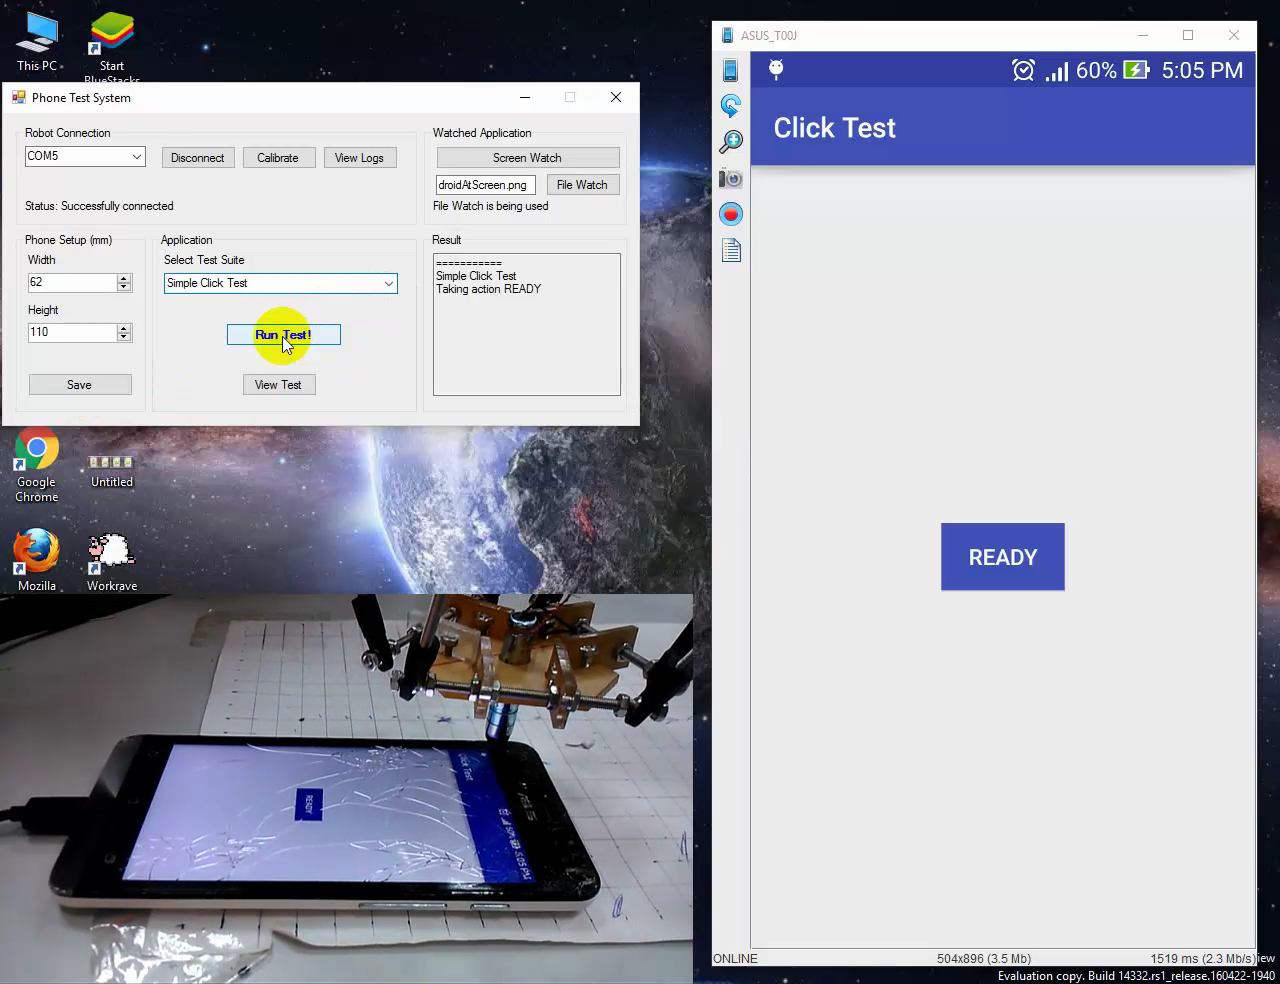
\includegraphics[width=\maxwidth{15cm}, keepaspectratio]{Chapters/Fig/click_start.png}
		\caption{Begin click test}
		\label{fig:click_start}
	\end{figure}
After clicking on READY, SUCCESS button appears. The robot is commanded to click on it. \\
Final result when READY is clicked. The test is Passed.
	\begin{figure}[H]
		\centering
		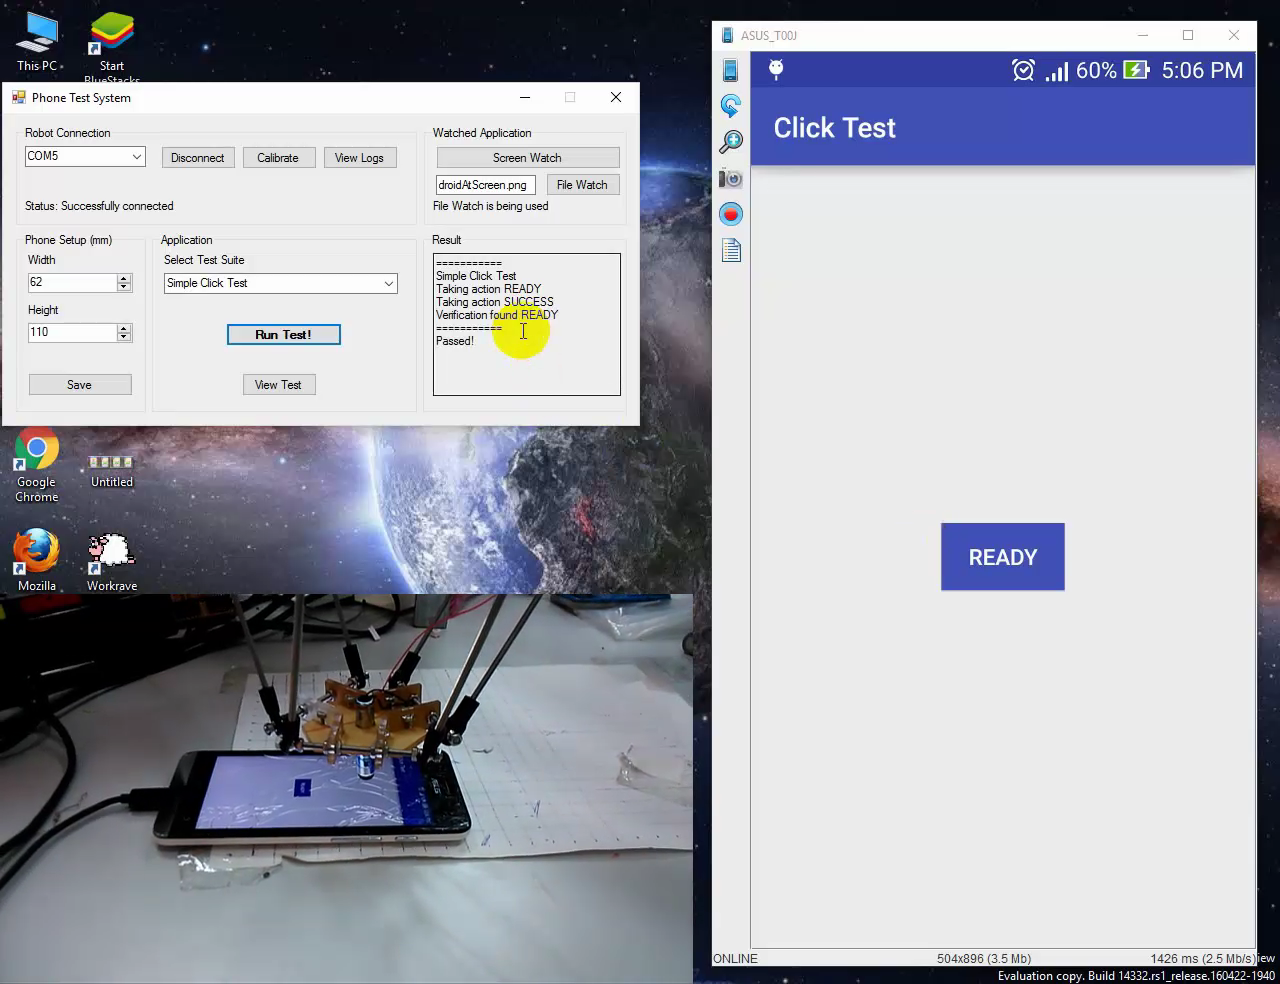
\includegraphics[width=\maxwidth{15cm}, keepaspectratio]{Chapters/Fig/click_final.png}
		\caption{Final click test}
		\label{fig:click_final}
	\end{figure}
\begin{table}[H]
	\centering
	\caption{Experiment 3: Test results statistic}	
	\label{tab:exp3_result_stat}
	\begin{tabular}{|lll|r|}
		\hline
		\textbf{Number of tests} & \textbf{Successful} & \textbf{Failed} & \textbf{Rate} \\
		\hline
		20 & 20 & 0 & 100$\%$\\
		\hline
	\end{tabular}
\end{table}
For simple task such as Simple Click, the system reaches absolute preciseness thus not any problem is made.

\subsection{Experiment 4: Combined Test 1: Set Alarm}
\subsubsection{Experiment's purpose}
Based on experiment control Delta robot select and setup alarm, I can test all the touch and swipe action
\subsubsection{Experimental setup}
	\begin{itemize}
		\item[--]Open Clock ICS application on the phone. Switch to Alarms screen of the application.
		\item[--]Follow the experimental procedure in previous section.
	\end{itemize}

\subsubsection{Experimental result and evaluations}
Before running the test, initial alarms are 8:30 AM and 9:00 AM. The goal of the test is to change 8:30 AM to 11:30 AM.
	\begin{figure}[H]
		\centering
		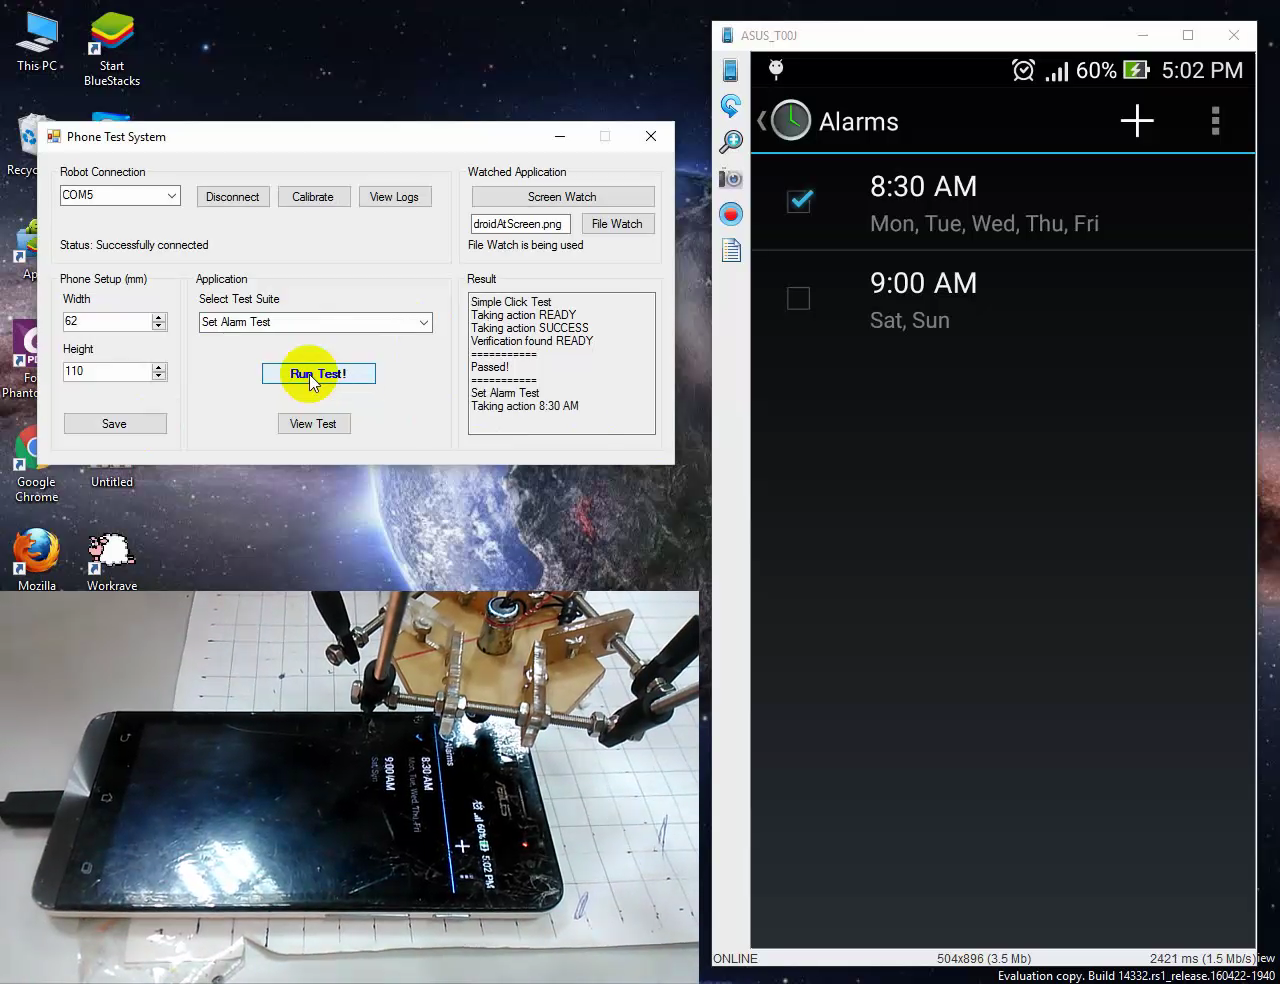
\includegraphics[width=\maxwidth{15cm}, keepaspectratio]{Chapters/Fig/alarm_start.png}
		\caption{Begin alarm test}
		\label{fig:alarm_start}
	\end{figure}
After proceeding some operations, the final screen of the application is shown below. 11:30 AM shows up and the test is successfully passed.
	\begin{figure}[H]
		\centering
		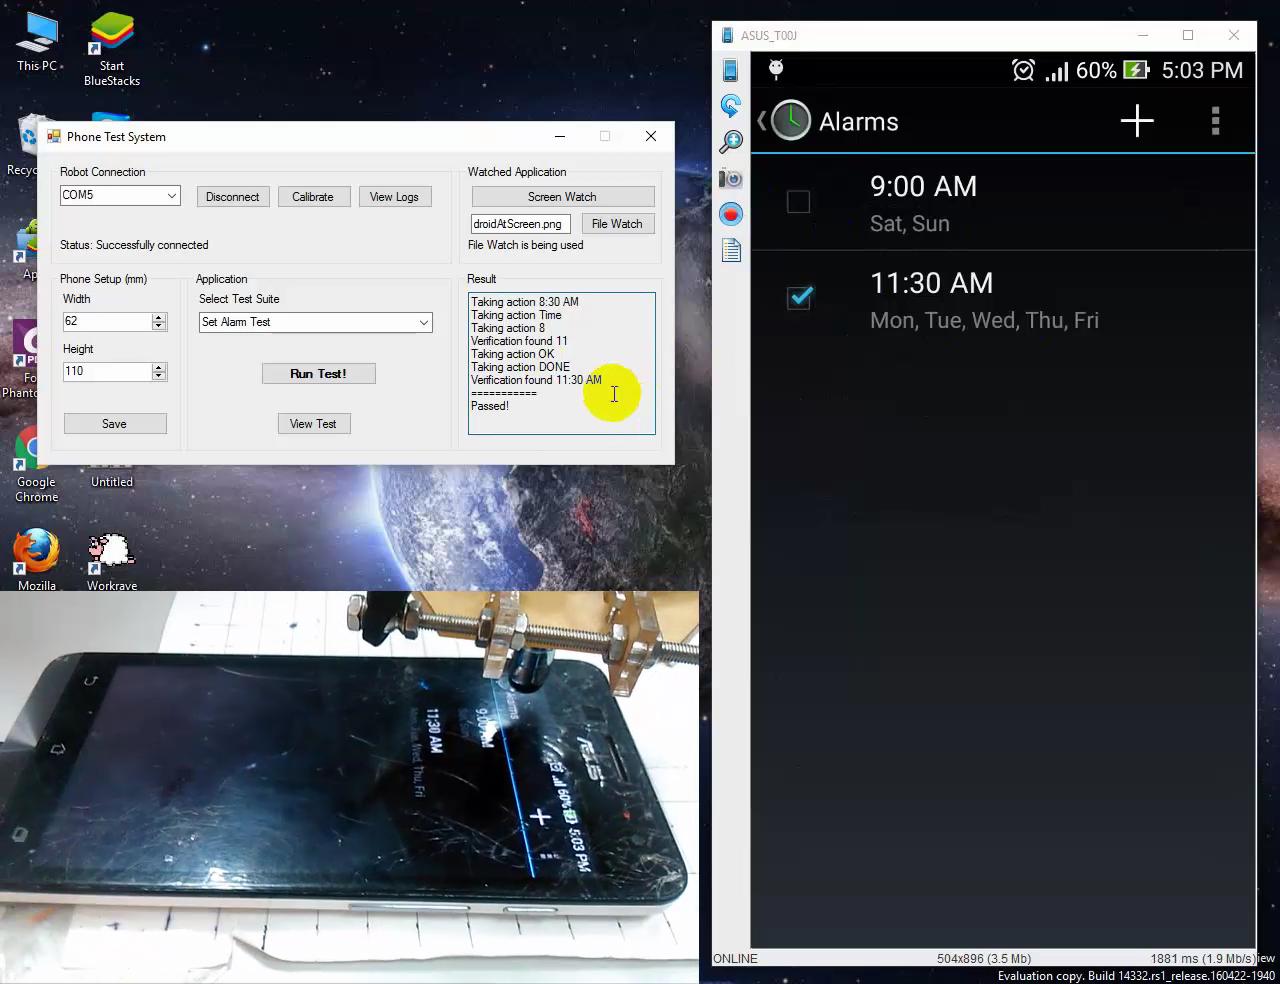
\includegraphics[width=\maxwidth{15cm}, keepaspectratio]{Chapters/Fig/alarm_final.png}
		\caption{Final alarm test}
		\label{fig:alarm_final}
	\end{figure}
\begin{table}[H]
	\centering
	\caption{Experiment 4: Test results statistic}	
	\label{tab:exp4_result_stat}
	\begin{tabular}{|lll|r|}
		\hline
		\textbf{Number of tests} & \textbf{Successful} & \textbf{Failed} & \textbf{Rate} \\
		\hline
		10 & 6 & 4 & 60$\%$\\
		\hline
	\end{tabular}
\end{table}

In Set Alarm task, Delta robot completes precisely the swipe screen action.

\subsection{Experiment 5: Combined Test 2: Set alarm label}
\subsubsection{Experimental purpose}
This experiment is conducted to verify the high-demanded precision in clicking items.

In addition, this test can also be considered as a real test case for an alarm application on Android phones that the tester has to carry out before releasing the application to the market.

\subsubsection{Experimental setup}
Set up as Experiment 4.

\subsubsection{Experimental results}
Before running the test, initial alarms are 8:30 AM with no label.

	\begin{figure}[H]
		\centering
		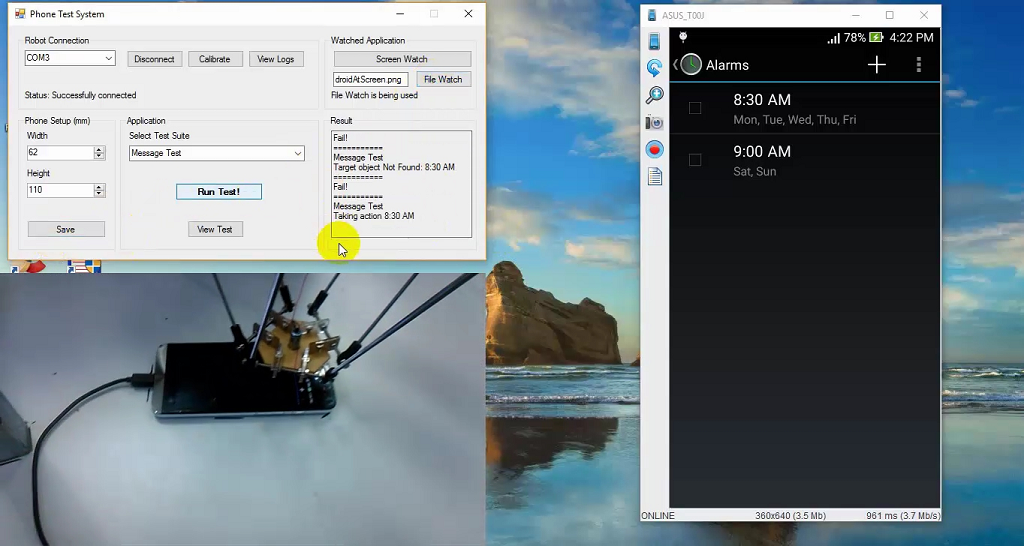
\includegraphics[scale=0.5]{Chapters/Fig/label_first.png}
		\caption{Begin typing test}
		\label{fig:label_first}
	\end{figure}

After proceeding some operations, the final screen of the application is shown below. 8:30 AM has label ``i love dce'' on the right. The test is successfully passed.

	\begin{figure}[H]
		\centering
		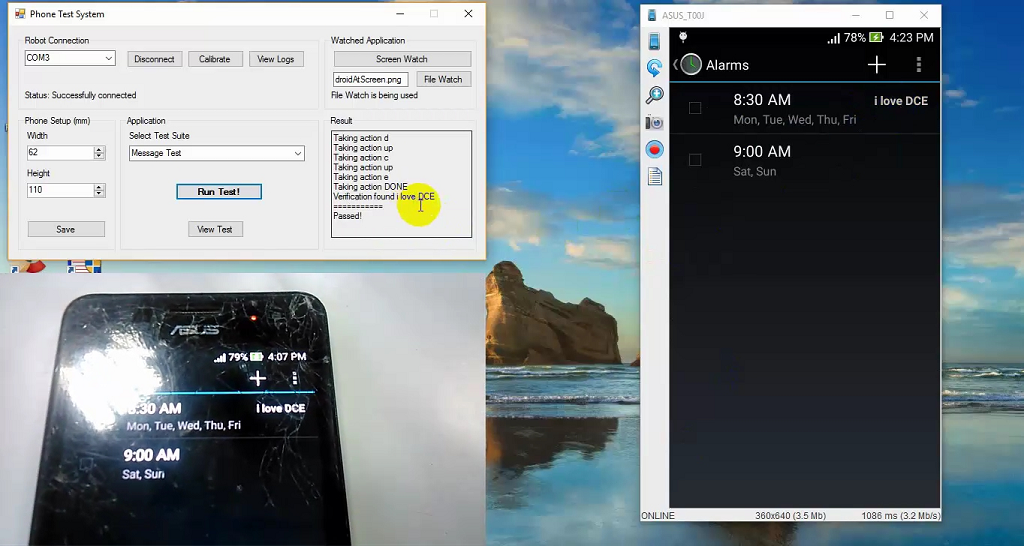
\includegraphics[scale=0.5]{Chapters/Fig/label_final.png}
		\caption{Final typing test}
		\label{fig:label_final}
	\end{figure}

\begin{table}[H]
	\centering
	\caption{Experiment 5: Set alarm label}	
	\label{tab:exp3_result_stat}
	\begin{tabular}{|lll|r|}
		\hline
		\textbf{Number of tests} & \textbf{Successful} & \textbf{Failed} & \textbf{Rate} \\
		\hline
		10 & 3 & 7 & 30$\%$\\
		\hline
	\end{tabular}
\end{table}

\section{Conclusion}
Throughout all experiment, the delta robot successfully pass all the automated testing case, which indicates it has a high accurately and stability moreover the robot work very well in the specified spatial working area ($4"\times6"$). This implies that my robot can be applied in real-world applications.

